\documentclass[../dissertation.tex]{subfiles}

\begin{document}

\subsection{Experiment 3 - Effects of CPU Clock Speed}
\label{experiment3-cpu-speed}

\paragraph{Introduction} During execution of Experiment 1, it was noted that higher message frequencies generally used a greater percentage of CPU time (using the Linux `top' utility). This gives rise to the possibilty that higher message frequencies cause higher latencies due to being CPU bound (meaning that the available processing power is not sufficient to process messages in a timely manner).

\paragraph{Objective} The purpose of this experiment was to identify whether the limited CPU power of the Raspberry Pi system was playing a significant role in the bottlenecking of message communication at higher frequencies. As in Experiment 2, this experiment has a secondary objective of further narrowing down the precise message frequency boundary that message latencies begin reducing - Experiment 2 identified this to be somewhere in the range between 1KHz and 4KHz.

\paragraph{Hypothesis} The hypothesis for the experiment was that frequencies which we had previously seen high message latency for would result in even higher latency, and the maximum `low latency' frequency would be lower as the core clock speed reduces.

\paragraph{Materials and Methodology} As in Experiment 2, the hardware platform is the same as presented in Experiment 1 (Section \ref{exp-1}). This experiment requires modifying the CPU speed of the host machines. This is achieved by underclocking the Raspberry Pi 3 Model B CPU by 25\%, and 50\%. The reason to do this instead of changing the hardware (for example changing to desktop machines) is that this method keeps variables such as CPU architecture, disk speed, and software stack the same across the experiment. It is also preferable to overclocking the Raspberry Pis (say to 125\%) as this can introduce a number of system instabilities (e.g. corrupted memory, or crashing) which can be difficult to detect. One potential issue is that modern CPUs often automatically underclock (reduce the clock speed and voltage) themselves, thus it can be hard to know exactly what CPU speed is being used throughout the experiment. Thus, several times throughout the experiment the current CPU speed was checked, and verified to be running at the specified maximum frequency. The exact method utilised to underclock the Raspberry Pis was to set the `arm\_freq' variable in the `/boot/config.txt' configuration file on the Raspberry Pis - the new clock speed then takes effect on the next reboot.

In order to give fine-grained results, many more message frequencies were tested than in previous tests. The experiment cycles through a range of message frequencies from 200Hz to 2Khz in 200Hz steps (e.g. 200Hz, 400Hz, ..., 1800Hz, 2000Hz). Three runs were conducted at each CPU speed, cycling through the entire frequency range each time. There was a 15 second waiting period between each message frequency run to allow for slow messages to clear the network before the next message frequency was run.

\paragraph{Results and Discussion} The results agreed with the hypothesis. At 100\% CPU clock speed, only the highest 3 frequencies showed sustained degradation of performance, however at 75\% the top 5 frequencies had increased message latencies, and at 50\% the top 7 had increased message latencies. Overall message latency was also increased as CPU core clock speed reduced. Even at the lowest frequency of 200Hz, 100\% CPU had an average message latency of 1.188ms, 75\%'s was 1.399, and 50\%'s was 1.609ms. Higher message frequencies demonstrated greater differences as shown in Figure \ref{exp3-averages}.

\begin{figure}[H]
\centering
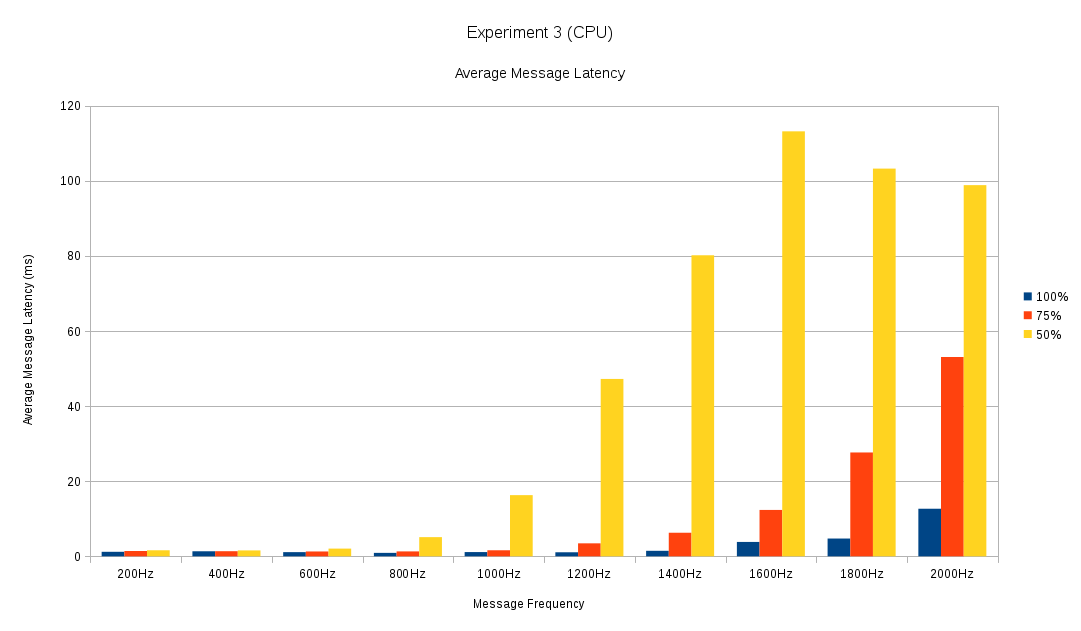
\includegraphics[width=\textwidth]{images/experiment3/average_per_frequency_graph.png}
\caption{Experiment 3 - All CPU Speeds, All Frequencies}
\label{exp3-averages}
\end{figure}

\begin{figure}[H]
\centering
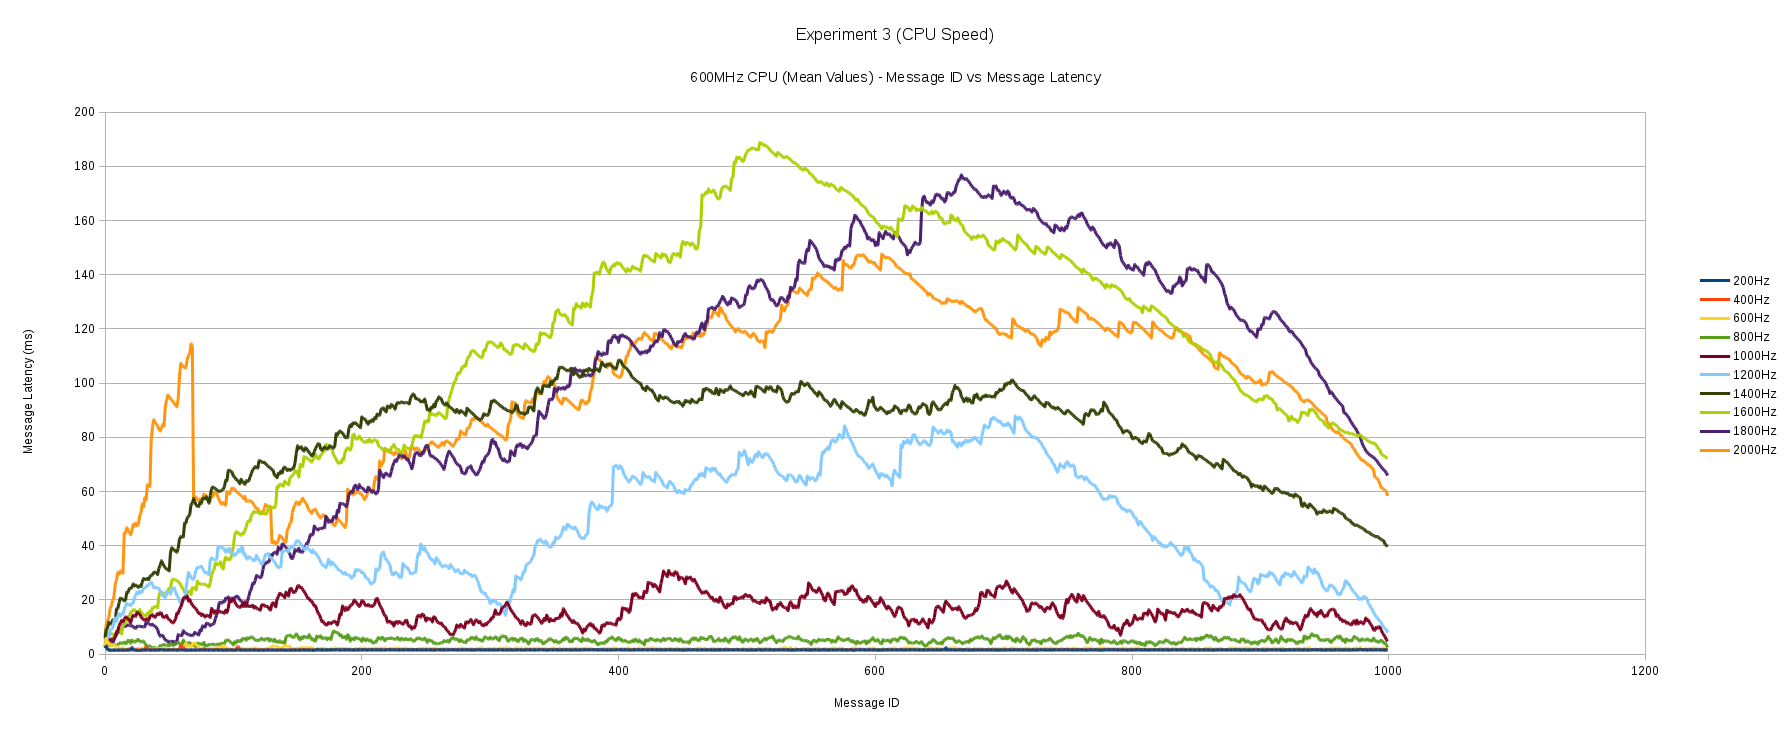
\includegraphics[width=\textwidth]{images/experiment3/50_clockspeed_mean_values_by_freq_pretty.png}
\caption{Experiment 3 - 50\% CPU Speed, All Frequencies}
\label{exp3-cpu100}
\end{figure}

\textit{We can conclude from these results that the CPU performance of the host machines can be a limiting factor for high frequency ROS communication, and thus CPU utilisation is an important metric when evaluating why a ROS system is experiencing poor performance. Secondly, we can conclude that for this test set-up and message size, at 100\% CPU speed the maximum sustainable message frequency is approximately 1400Hz.}

\end{document}
